\documentclass[12pt]{beamer}
\usetheme{Copenhagen}
\title{TCP Maquina de estados finitos}
\author{Antunez Joaquin, Gonzalez Alejo y Nielsen Maximiliano}
\date{\today}
\begin{document}
\begin{frame}
\titlepage
\end{frame}
\begin{frame}{Administración de conexiones}
\begin{figure}
	\centering
	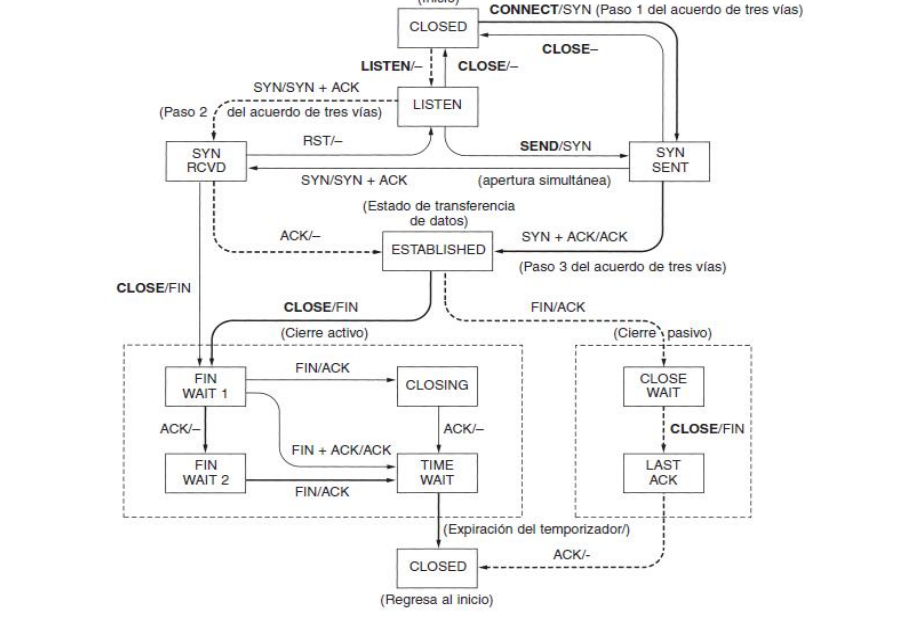
\includegraphics[width=0.7\linewidth]{Documents/Lab1(img)/pag1}
	\label{fig:fig1}

	\tiny Maquina de estados finitos de administración de conexiones TCP. La linea contunua
	gruesa es la trayectoria normal de un cliente. La linea punteada gruesa es la trayectoria normal de
	un servidor. Las lineas delgadas son eventos poco comunes. Cada trancisición está indicada por el 
	evento que la ocasiona y la acción resultante, separada por una diagonal
\end{figure}
\tableofcontents
\end{frame}
\begin{frame}{Administración de conexiones}
\small	La máquina de estados finitos del slide anterior . El caso común de un cliente que
	se conecta activamente a un servidor pasivo se indica con líneas gruesas
	(continuas para el cliente, punteadas para el servidor). Las líneas delgadas son
	secuencia de eventos poco comunes. Cada línea de la figura se marca mediante
	un par evento/acción.\\
	\vspace{7mm}	
	El evento puede ser una llamada de sistema iniciada por el usuario (CONNECT,
	LISTEN, SEND o CLOSE), la llegada de un segmento (SYN, FIN, ACK o RST) o,
	en un caso, una expiración de temporizador del doble del tiempo de vida máximo
	del paquete.\\
	\vspace{7mm}	
	La acción es el envío de un segmento de control (SYN, FIN
	o RST), o nada, indicado por —. Los comentarios aparecen entre paréntesis.
\end{frame}
\begin{frame}{Liberación y Establecimiento de una conexión}	
\begin{figure}
	\centering
	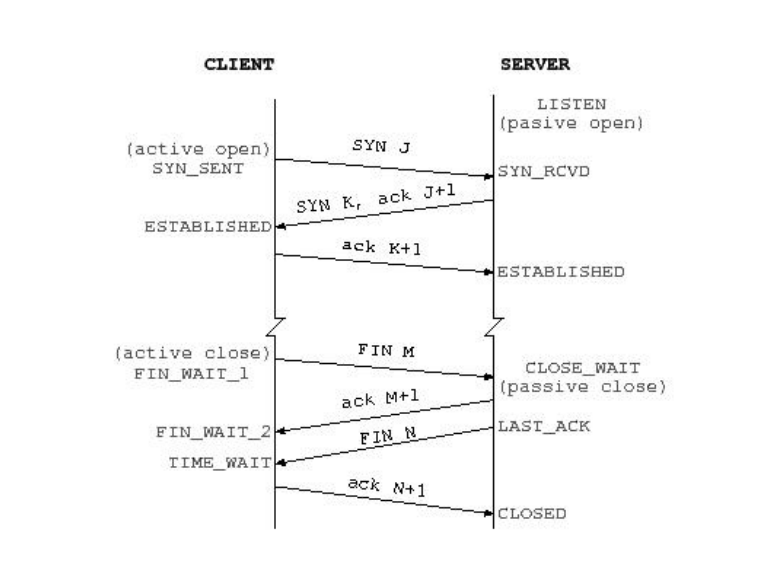
\includegraphics[width=1\linewidth]{Documents/Lab1(img)/img2}
	\label{fig:img2}
\end{figure}
\end{frame}
\begin{frame}{TCP: Maquina de estados finitos}	
	\begin{figure}
		\centering
		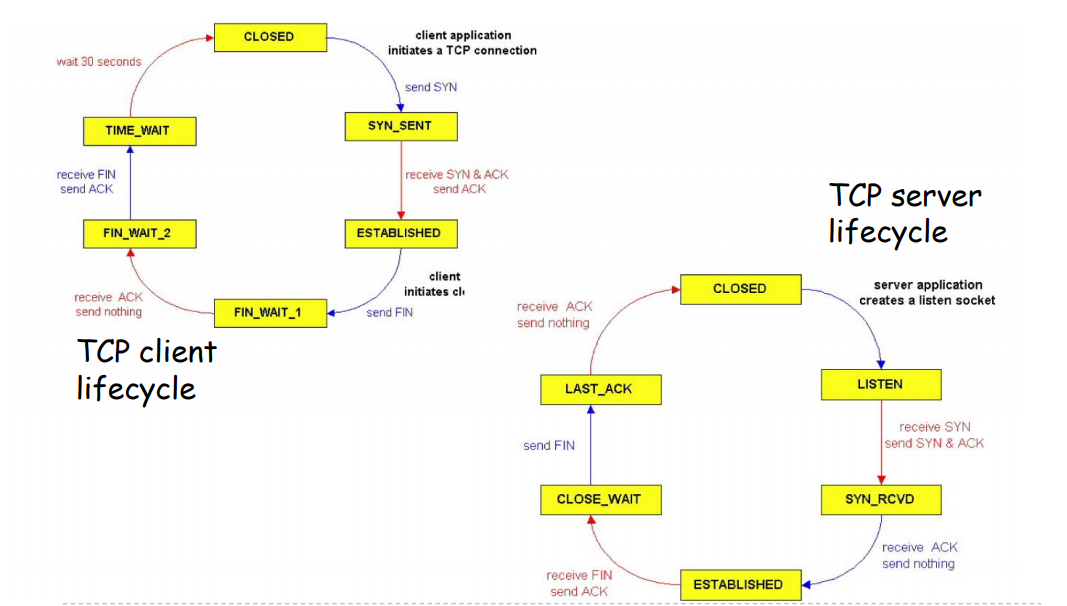
\includegraphics[width=1.1\linewidth]{Documents/Lab1(img)/img3}
		\label{fig:img3}
	\end{figure}
\end{frame}
\begin{frame}{Estados del Modelo TCP}	
\begin{table}[]
	\begin{tabular}{|l|c|}
		\hline
		\textbf{Estado}&\textbf{descripcion}  \\ \hline
	CLOSED&No hay conexión ni activa ni pendiente  \\ \hline
	LISTEN&El servidor espera una llamada  \\ \hline
	SYN RCVD&Llegó solicitud de conexión;espera ACK  \\ \hline
	SYN SENT&La aplicación comenzó a abrir una conexión  \\ \hline
	ESTABLISHED&Estado normal de transferencia de datos  \\ \hline
	FIN WAIT 1& La aplicacion dijo que ya terminó \\ \hline
	FIN WAIT 2& El otro lado acordó liberar \\ \hline
	TIMED WAIT& Espera que todos los paquetes mueran \\ \hline
	CLOSING&Ambos lados intentaron cerrar simultáneamente  \\ \hline
	CLOSE WAIT& El otro lado inició una liberación \\ \hline
	LAST ACK&Espera que todos los paquetes mueran  \\ \hline
	\end{tabular}
\end{table}
\end{frame}
\begin{frame}{Liberación “Tear-down”}	
	\begin{figure}
		\centering
		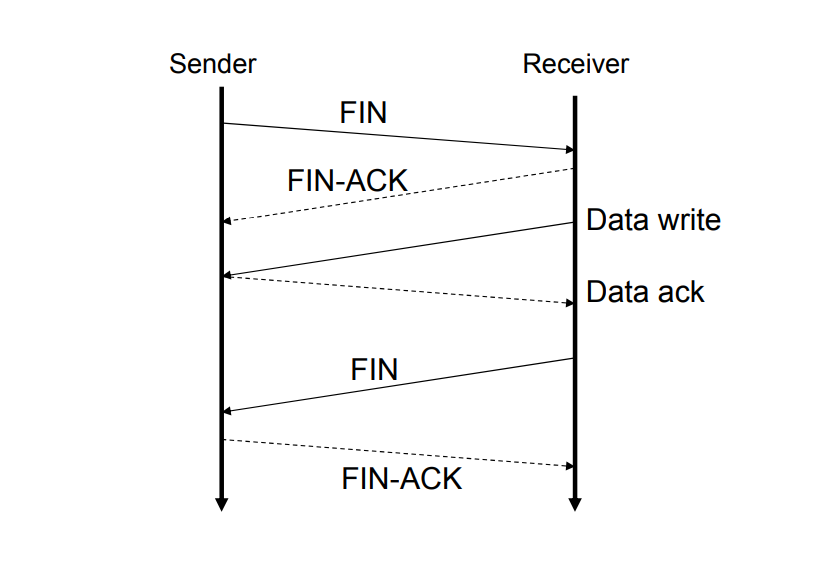
\includegraphics[width=1\linewidth]{Documents/Lab1(img)/img4}
		\label{fig:img4}
	\end{figure}
\end{frame}
\begin{frame}{Conexión “Tear-down}	
	\begin{figure}
		\centering
		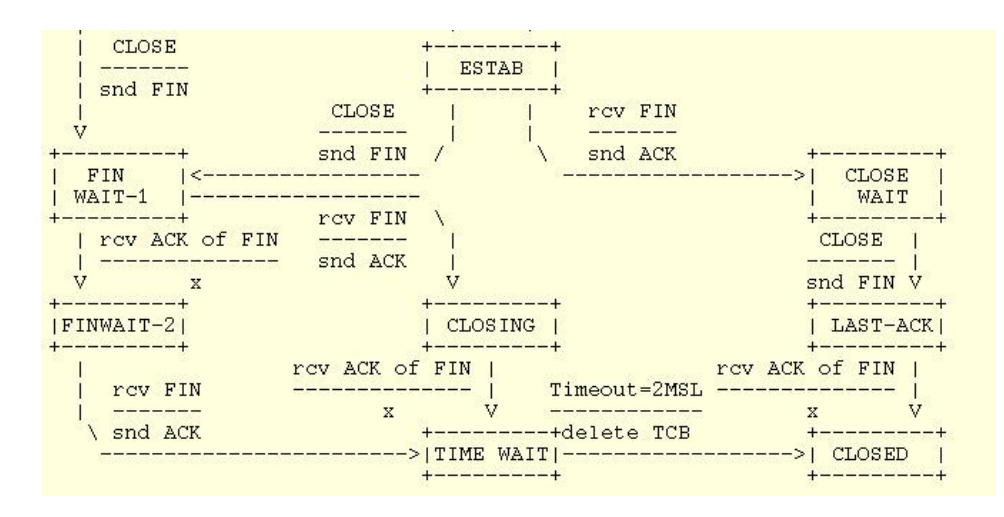
\includegraphics[width=1\linewidth]{Documents/Lab1(img)/img5}
		\label{fig:img5}
	\end{figure}
\end{frame}
\begin{frame}{Detectando “Half-open Connections”}	
	\begin{figure}
		\centering
		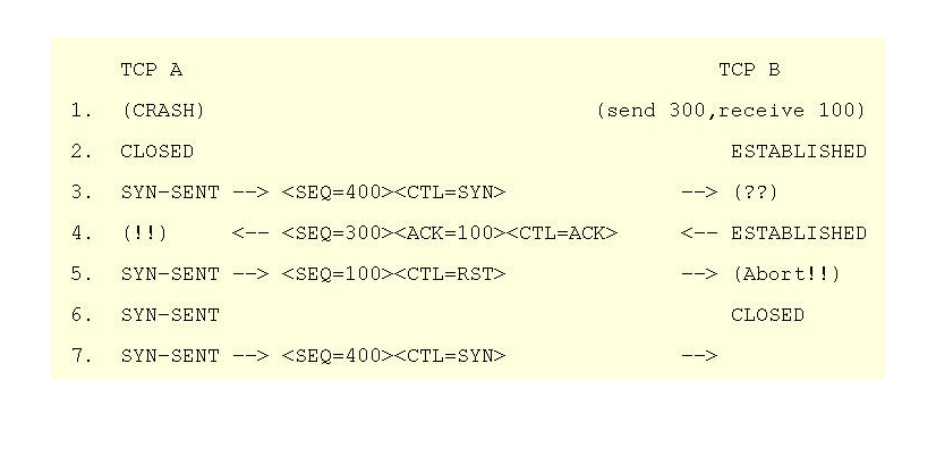
\includegraphics[width=1\linewidth]{Documents/Lab1(img)/img6}
		\label{fig:img6}
	\end{figure}
\end{frame}
\begin{frame}{TIME-WAIT Assassination}	
	\begin{figure}
		\centering
		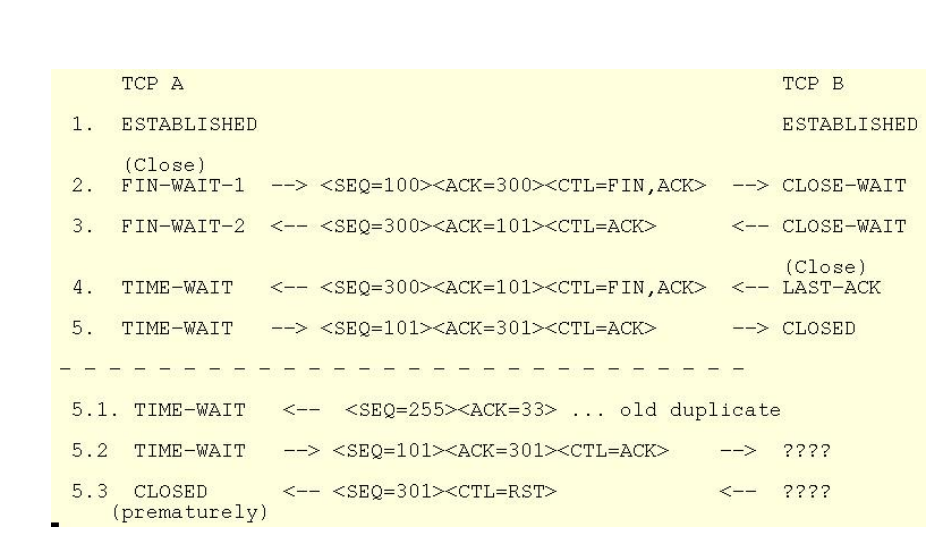
\includegraphics[width=1\linewidth]{Documents/Lab1(img)/img7}
		\label{fig:img7}
	\end{figure}
\end{frame}
\end{document}